\documentclass[]{report}
\usepackage{listings}
\usepackage[margin=1.25in]{geometry}
\usepackage{graphicx}
\usepackage{pdfpages}


% Title Page
\title{PART A \\ PART 2 \\ Comparing the Performance of Implicit and Explicit Concurrency in Java}
\author{Dominic Rathbone}


\begin{document}
\maketitle

\section*{Introduction}
In order to compare the effects of concurrency on performance of a Java application, A test program was created that compared various implementations of concurrency, implicit and explicit, to a baseline non-concurrent implementation. These implementations performed a mathematical operation finding all the mersenne primes in a set of integers derived from the user inputting a start and end number at launch. Time (in nano seconds) was used as a benchmark in order to compare these implementations. The time was taken before and after each implementation ran and then the total run time was derived from them. In order to compare them with ease, a ratio derived from dividing the total time of the baseline implementation by the total time of concurrent implementation is outputted to csv files. To run the programs, A ThinkPad laptop running Fedora with a quad-core 2.50GHz i5-2520M CPU and 8 gigabytes of RAM was used as well as a Gaming PC running Windows 7 with a quad-core 3.50GHz i5 4690K and 8 gigabytes of RAM.

\section{Non-concurrent Approach}
The non-concurrent approach runs the operations sequentially, running over the sequence of integers with a for statement and incrementing a counter every time a prime number is found. This is used as the baseline to compare the implicit and explicit concurrent approaches to.(see Appendix A)

\section{Multi-threading}
The first explicitly concurrent implementation uses raw threads to run the operation over the sequence of numbers. This was attempted in two ways. First of all, to make the test a better comparison, I produced an implementation that spawned a new thread for every number in the sequence (see Appendix B, figure 1), similar to how a parallel stream would split a stream of numbers into multiple parallel sub-streams. On testing this implementation, it was revealed that this would not be an efficient way to approach concurrency because as the sequence of numbers became larger, it would become extremely slow (finishing minutes where other approaches finished in seconds). This was due to the lack of thread management such as a queue or limit to how many threads should be started at once meaning the machine bottlenecked by a flood of threads. As a result of this, the implementation was re-factored and it was decided that the best way to approach this was to split the sequence of numbers down into smaller sequences using the number of cores with one subsequence per thread per core (see Appendix B, figure 2). This would mean that although each CPU core had to process with a larger sequence of numbers per thread, the number of threads and the overhead associated with them was lower making the time drastically faster.
 
\section{Thread Pooling}
The second explicitly concurrent implementation was through the use of thread pools and futures. A thread pool is a group of pre-defined threads that can be used to run tasks. In this approach, a task is submitted to the thread pool for every number in the sequence. This is similar to the raw multi-threaded implementation but the thread pool can queue the threads so they do not start at the same time and bottleneck the machine as mentioned in the previous section. The results of this task is then retrieved through a "Future", an object that represents the results from the submission of the task (see Appendix C).

\section{Streaming}
This approach takes the sequence of number and processes it as a stream, applying intermediate operations on each element in the stream until it reaches an terminal operation which ends the set of operations. This can be done sequentially with a serial stream (see Appendix D) or concurrently with a parallel stream (see Appendix E). The result set includes both serial and parallel stream in order to compare how they perform.

\section{Data Analysis}

From the data (Appendix F), we can see that running the program on the desktop PC gave better results on average compared with running them on the laptop with the highest ratio for each concurrent implementation running on PC being 1.5x to 2x faster than on the laptop and the average ratio being 1.5x faster on the PC than on the laptop. This implies that all of these concurrent implementations do scale with hardware and that, vice versa, worse hardware will bottleneck concurrent applications. However, there are other variables that could have affected the performance such as other processes using the CPU during the period the program was running or the different operating system that the tests were being ran on (Windows 7 \& Fedora 22).

Across the implementations, on both PC and laptop, it can be seen that on average, The raw multi-threaded approach and the parallel stream were faster compared to the baseline than the thread pool approach especially as the size of data set got larger. However, the graphs (Appendix G) indicate that on both machines, as the end value got larger, the thread pool can be seen to improve dramatically in performance, in particular when the end value reached 801million. This could imply that the programs were not ran over a data set with a large enough end value and that the thread pool may actually perform just as well or better as the numbers increased past this point. This is especially worth noting as the highest ratio (1:3.7972339477 on PC, 1:2.0458180569 on laptop) from the thread pool data found at the 800-801 million data set is higher than the highest ratio from the parallel stream approach (1:3.5239193257 on PC, 1:2.0271960552 on laptop). On the other hand, if we look at the graph mapping the size of the data set to performance, the thread pool approach seems to peak at a size of 1,000,000 to 3,000,000 and then drop as the size increases past this point implying that although it may perform at larger numbers, performance might decrease as the distance between the start value and the end value gets larger. 

It can be seen from the graphs (Appendix G) that, across all concurrent implementations and machines, as the end value of the data sets increased, the performance initially increased until a plateau was reached at around the size of 200000. The increase could be because as the numbers got larger, the cost of the overhead of running the tasks concurrently in each implementation was outweighed by the benefits of calculating these tasks in this manner. The plateau implies that the software reached a point where hardware limitations such as the number of cores started to bottleneck the program. 

One unusual result was how the performance of the multi-threaded approach spiked twice very early on in the graph which is surprising as the cost of using threads on data sets this small usually outweighs the benefit. This occurred on both the desktop PC and the laptop results which implies that it isn't caused by something machine-specific. 

Overall, the results reflected what was expected from the tests with the exception of the thread pool approach, of which I expected to be faster than the multi-threaded approach due it's thread management capabilities. However, due to how I re-factored the multi-threaded approach to split the sequence of numbers differently, it may not be fair to compare the two. If I were to leave the multi-threaded implementation to run the operations in a similar manner to the thread-pool, it would most likely vastly be out-performed.

\appendix
\chapter{}
\begin{figure}[h!]
	\caption{Non-concurrent}
	\begin{lstlisting}[language=Java,frame=single]
public static void nonConcurrent() {
	for ( long n = START; n < END; n++ ) {
		int primeCount = 0;
		if (Calculator.isMersennePrime(n)) {
			primeCount++;
		}
	}
}
	\end{lstlisting}
\end{figure}

\chapter{}
\begin{figure}[h!]
	\caption{Multi-threaded 1}
	\begin{lstlisting}[language=Java,frame=single]
public static void multiThreaded() {
	List<Thread> threads = new ArrayList<>();
		for (long n = START; n < END; n++) {
			Thread thread = new Thread(
				new RunnableA(n)
			);
			thread.start();
			threads.add(thread);
		}
		for(Thread thread: threads) {
			try {
				thread.join();
			} catch (InterruptedException e){
				e.printStackTrace();
			}
		}
}
	\end{lstlisting}
\end{figure}

\begin{figure}[h!]
	\caption{Multi-threaded 2}
	\begin{lstlisting}[language=Java,frame=single]
public static void multiThreaded2() {

	List<Thread> threads = new ArrayList<>();
	long subsequence = (END - START) / CORES;
	
	for ( long n = START; n < END; n=n+subsequence) {
		Thread thread = new Thread(
			new RunnableB(n, n+subsequence)
		);
		thread.start();
		threads.add(thread);
	}
	
	for(Thread thread: threads) {
		try {
			thread.join();
		} catch (InterruptedException e) {
			e.printStackTrace();
		}
	}
}
	\end{lstlisting}
\end{figure}

\chapter{}
\begin{figure}[h!]
	\caption{Thread Pool}
	\begin{lstlisting}[language=Java,frame=single]
public static void threadPool() {
	ExecutorService executorService =
		Executors.newFixedThreadPool(CORES);
	ArrayList<Future<Integer>> futures =
		new ArrayList<>();
	
	for ( long n = START; n < END; n++ ) {
		final long number = n;
		Future<Integer> future =
		executorService.submit(() -> {
		  if(Calculator.isMersennePrime(number)) {
			  return 1; 
		  }
		  else {
			  return 0;
		  }
		}
		);
		futures.add(future);
	}
	
	int primeCount = 0;
	for (Future<Integer> future : futures) {
		try {
			primeCount += future.get();
		} catch (Exception e) {
		}
	}
	executorService.shutdown();
}
	\end{lstlisting}
\end{figure}

\chapter{}
\begin{figure}[h!]
	\caption{Serial Stream}
	\begin{lstlisting}[language=Java,frame=single]
public static void serialStream() {
	long primeCount = Stream
	.iterate(START, n -> n + 1)
	.limit(END-START)
	.filter( n -> Calculator.isMersennePrime(n) )
	.count();
}
	\end{lstlisting}
\end{figure}
\chapter{}
\begin{figure}[h!]
	\caption{Parallel Stream}
	\begin{lstlisting}[language=Java,frame=single]
public static void parallelStream() {
	long primeCount = Stream
	.iterate(START, n -> n + 1)
	.limit(END-START)
	.parallel()
	.filter(n -> Calculator.isMersennePrime(n) )
	.count();
}
	\end{lstlisting}
\end{figure}

\chapter{}
	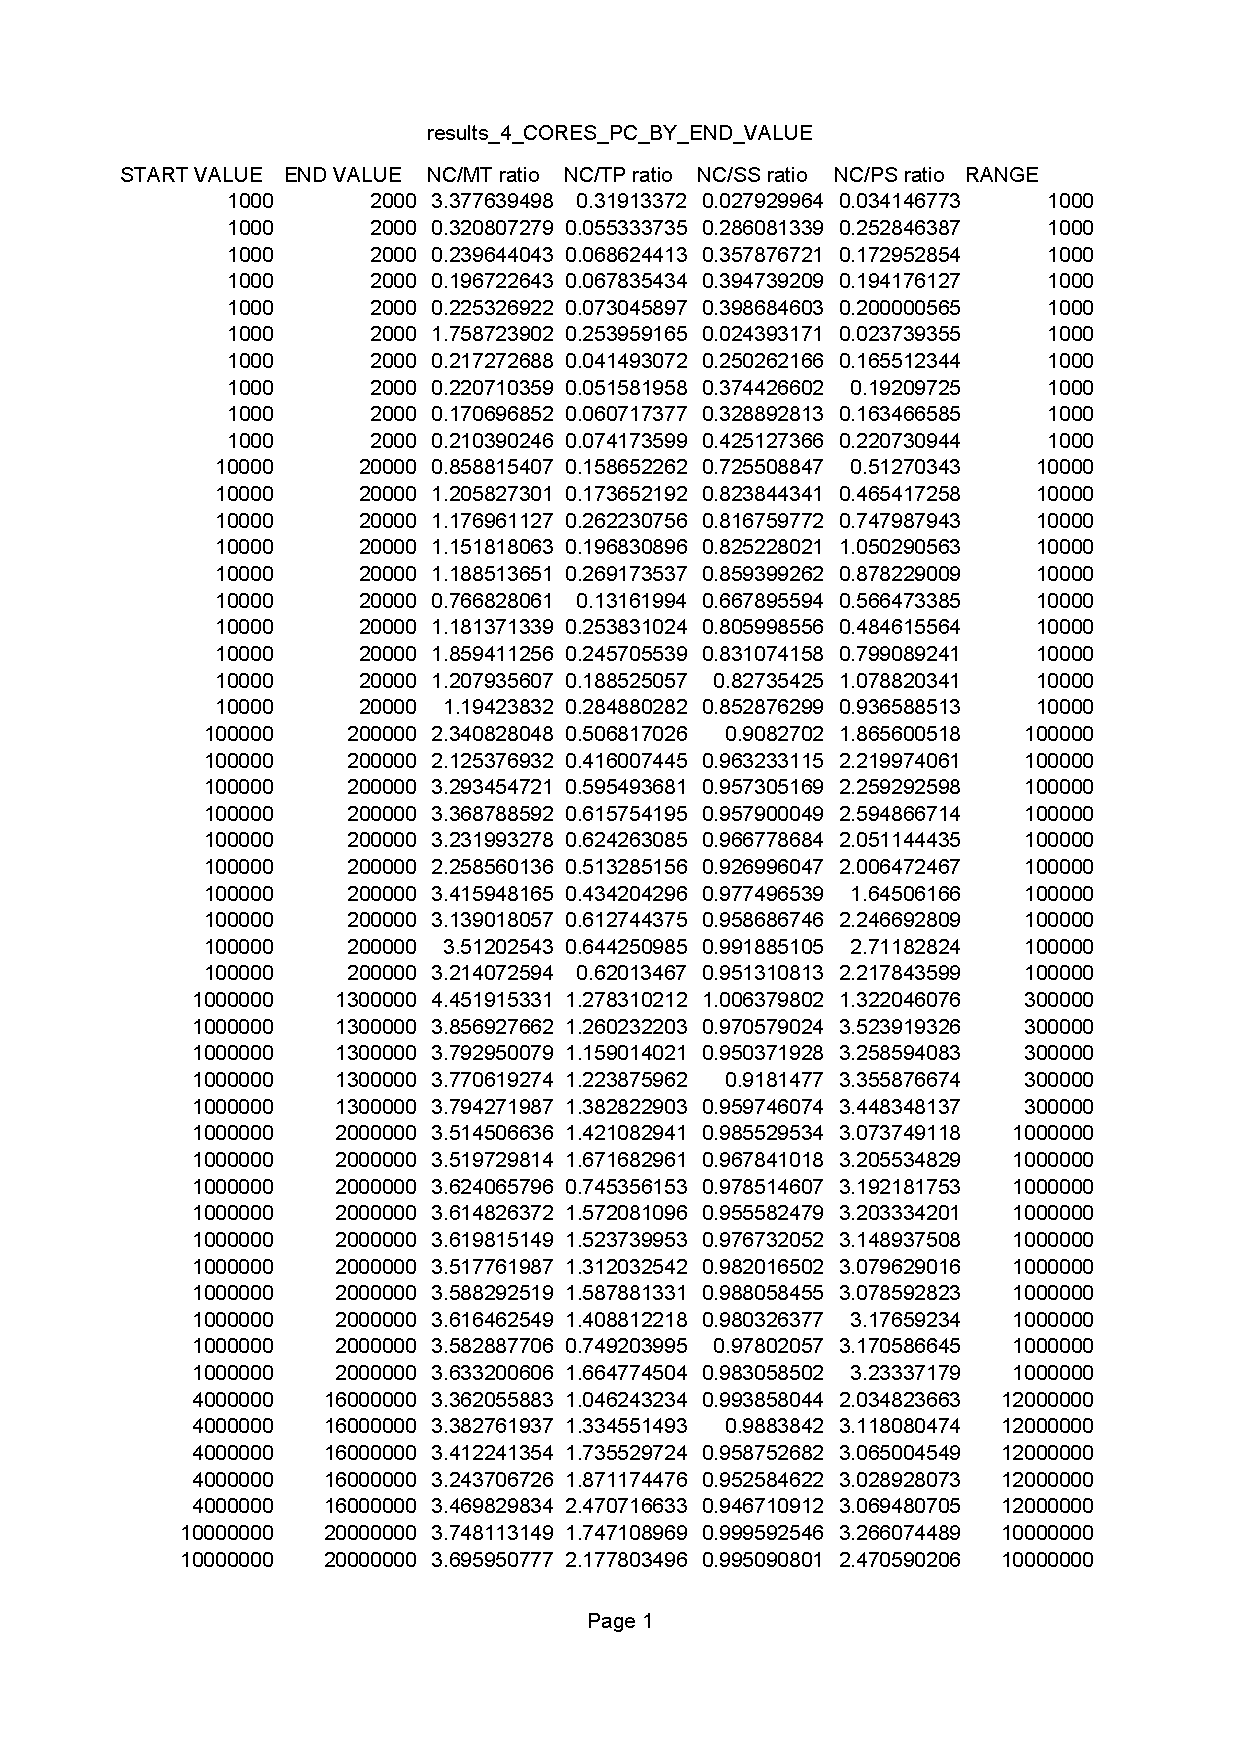
\includepdf[pages={1}]{results_4_CORES_PC.pdf}	
	\includepdf[pages={2}]{results_4_CORES_PC.pdf}	
	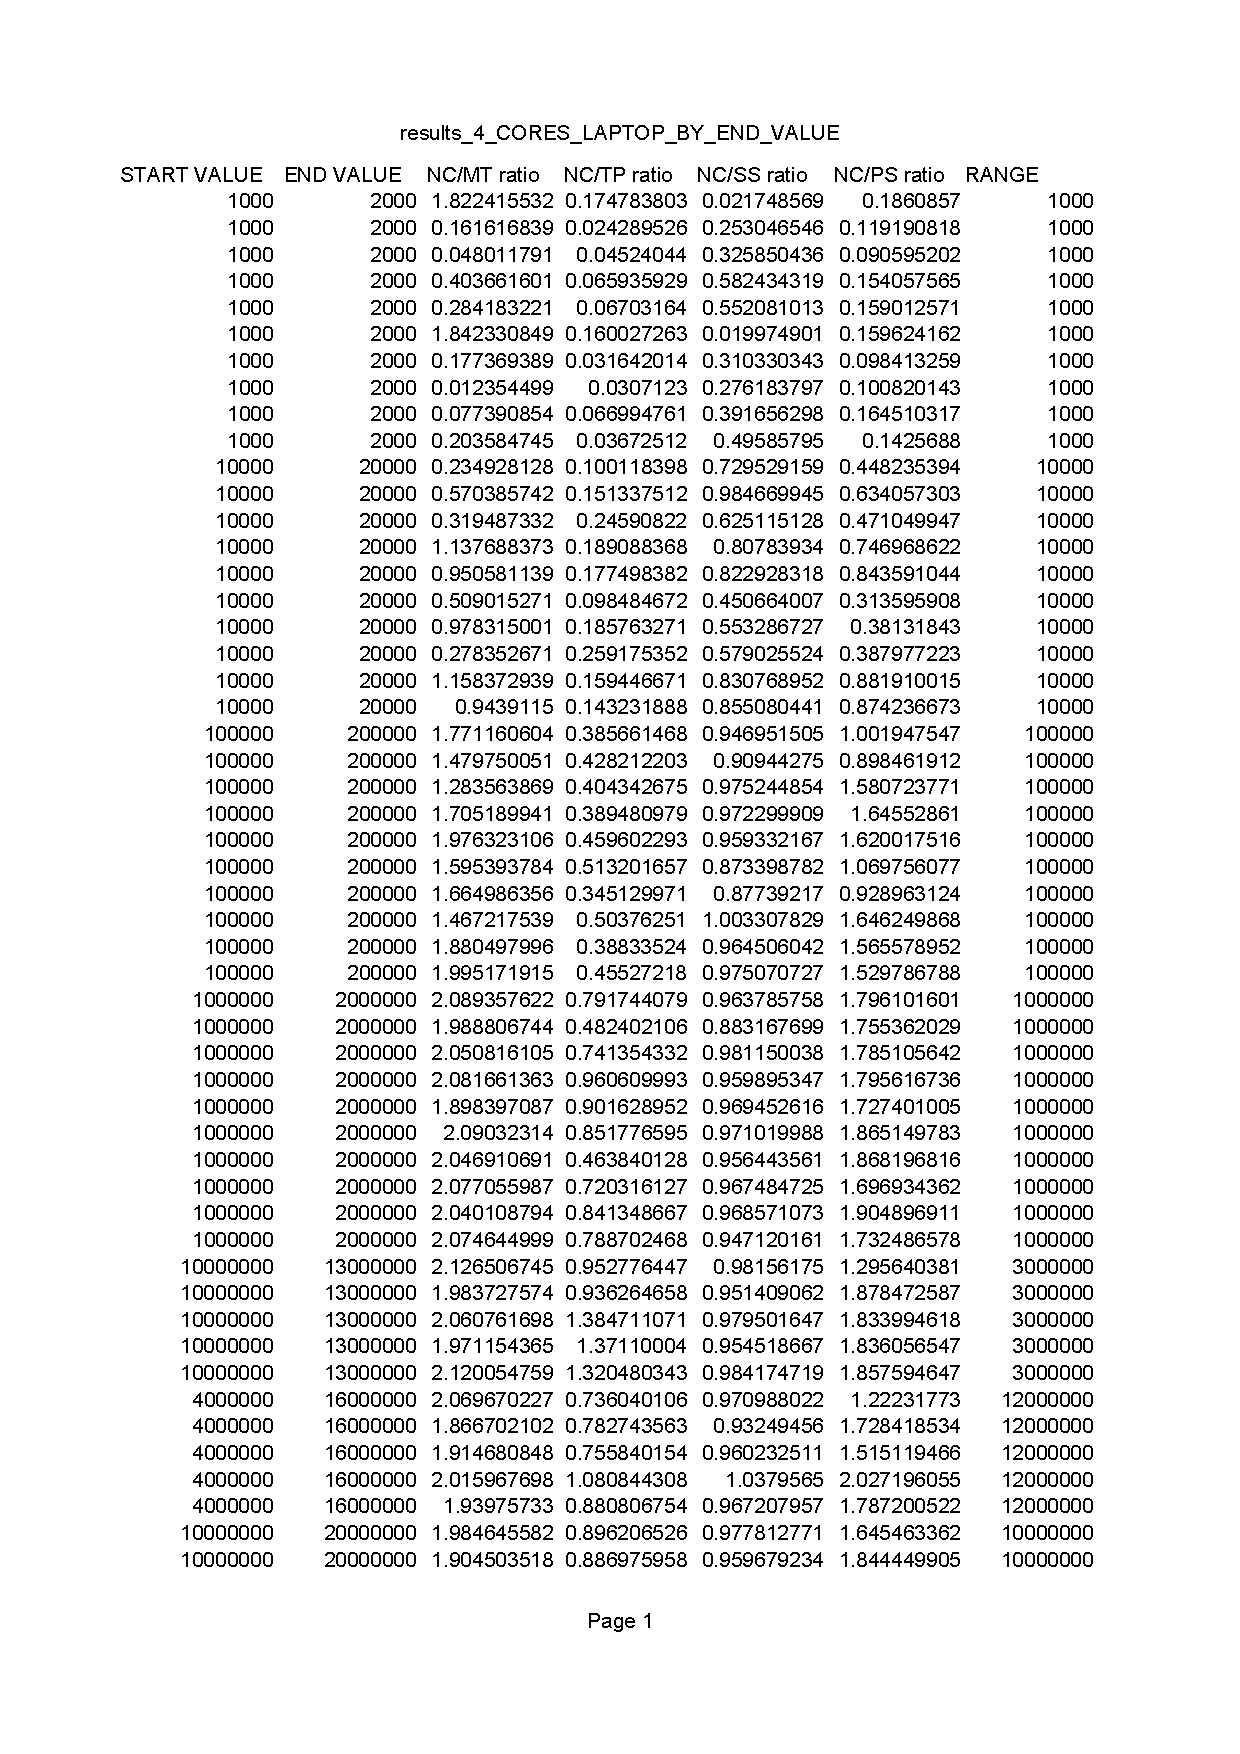
\includepdf[pages={1}]{results_4_CORES_LAPTOP.pdf}
	\includepdf[pages={2}]{results_4_CORES_LAPTOP.pdf}
	
\chapter{}
\begin{figure}[h!]
	\caption{PC Results}
	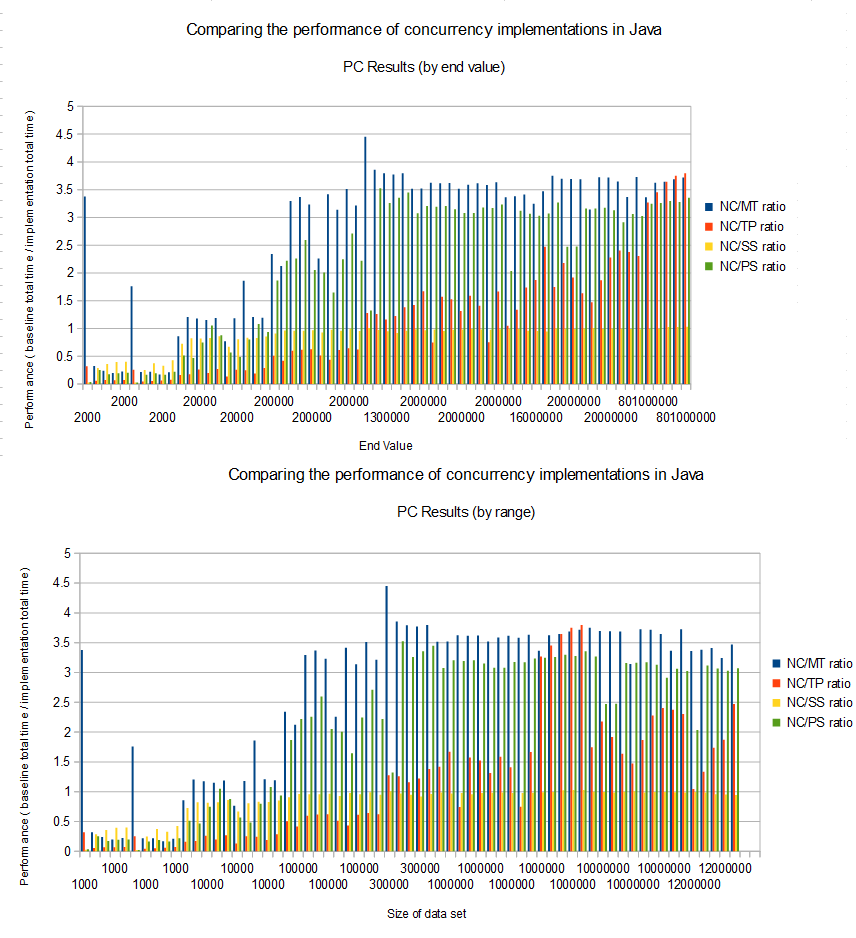
\includegraphics[scale=0.75]{PC_GRAPHS.png}
\end{figure}

\begin{figure}[h!]
	\caption{Laptop Results}
	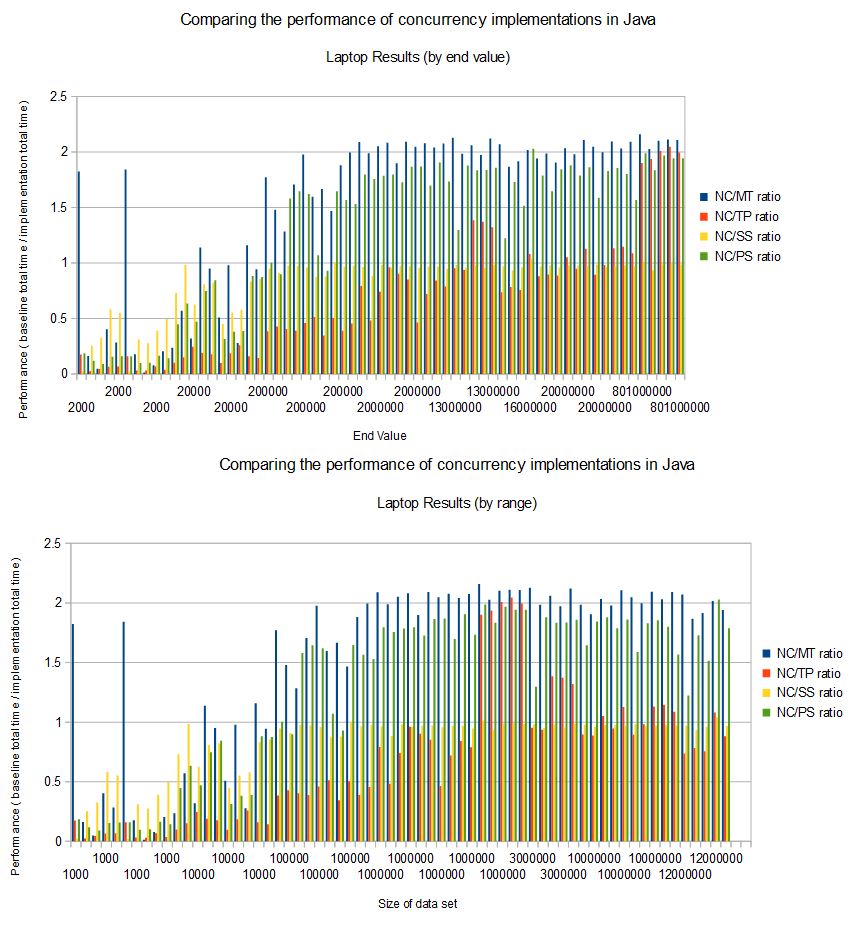
\includegraphics[scale=0.75]{LAPTOP_GRAPHS.png}
\end{figure}
\end{document}          
